\chapter{CÀI ĐẶT MINH HỌA}

\section{Dữ liệu thực nghiệm và thiết lập hệ thống}

Nhóm đánh giá bốn hệ thống trên \textbf{Spider 1.0 dev} \cite{ref7} gồm 1.034 câu hỏi tiếng Anh trên 20 CSDL SQLite, chia theo độ khó của gold SQL: \textbf{Easy} 248, \textbf{Medium} 446, \textbf{Hard} 174 và \textbf{Extra} 166 câu. Tập train\_spider (7.000 câu, 140 CSDL) là kho ví dụ \emph{few-shot} cho DAIL-SQL (không \emph{fine-tune}). Cả bốn hệ thống chạy trên cùng danh sách câu hỏi: DIN-SQL, DAIL-SQL và MAC-SQL dùng cx/gpt-6-luna; Codex MCP SQL chạy trên Codex SDK (v0.163.0, effort low) với gpt-6-luna. Mã nguồn: \url{https://github.com/dleqhuy/text2sql-comparison}.

\section{Pipeline các phương pháp thực nghiệm}

Theo Bảng III \cite{ref1}, DIN-SQL, MAC-SQL thuộc C1+C4; bản DAIL-SQL của nhóm chỉ dùng C2 (Hình 4.1):

\begin{figure}[htbp]
\centering
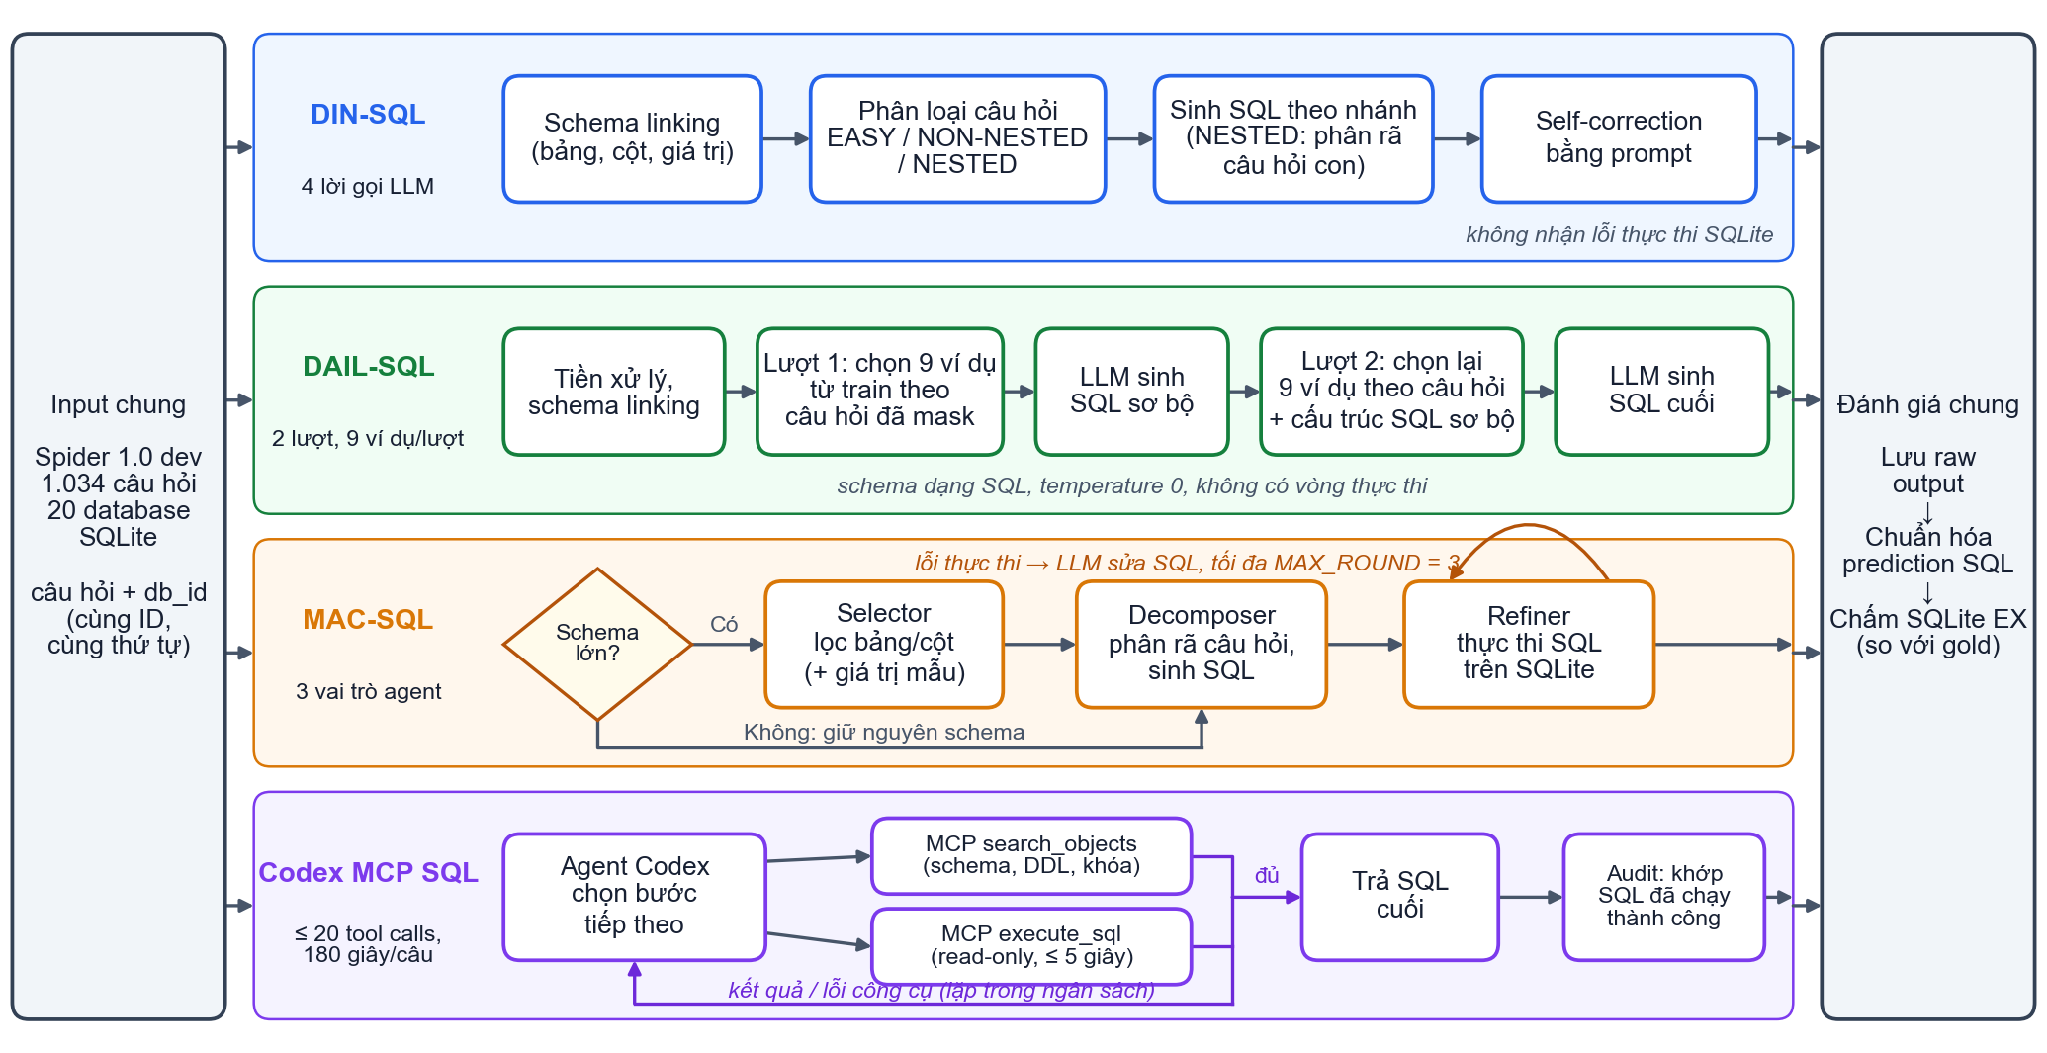
\includegraphics[width=\linewidth,height=0.68\textheight,keepaspectratio]{05-experimental-pipelines}
\caption{Pipeline thực nghiệm của bốn phương pháp Text-to-SQL}\label{fig:05-experimental-pipelines}
\end{figure}

\begin{itemize}
\item \textbf{DIN-SQL \cite{ref4} (phân rã tuần tự):} Schema Linking, phân loại câu hỏi (EASY, NON-NESTED, NESTED), sinh SQL theo \emph{prompt} của từng nhánh (NESTED có phân rã câu hỏi con) và \emph{self-correction} bằng \emph{prompt}, temperature 0; không nhận lỗi thực thi.
\item \textbf{DAIL-SQL \cite{ref5} (chọn ví dụ few-shot hai lượt):} biểu diễn \emph{schema} dạng SQL; lượt 1 chọn 9 ví dụ theo \emph{Euclidean distance} của câu hỏi đã \emph{mask} để sinh SQL sơ bộ; lượt 2 chọn lại 9 ví dụ theo câu hỏi và cấu trúc SQL sơ bộ; không có vòng sửa lỗi thực thi.
\item \textbf{MAC-SQL \cite{ref6} (multi-agent có phản hồi lỗi):} Selector lọc \emph{schema} lớn kèm giá trị mẫu; Decomposer phân rã câu hỏi và sinh SQL; Refiner thực thi trên SQLite và sửa theo thông báo lỗi (tối đa MAX\_ROUND = 3).
\item \textbf{Codex MCP SQL (nhóm xếp vào C3 tool-augmented và C4):} \emph{agent} gọi search\_objects (khám phá DDL, \emph{schema}) và execute\_sql (read-only, \ensuremath{\leq} 5 giây), ngân sách \ensuremath{\leq} 20 \emph{tool calls} và 180 giây/câu; SQL cuối phải khớp một truy vấn đã chạy thành công.
\end{itemize}

\section{Kết quả thực nghiệm và phân tích đối sánh}

Dự đoán của bốn hệ thống được chấm bằng đủ bốn độ đo của Mục III-B \cite{ref1} trên cùng 1.034 câu: \textbf{EX} thực thi trên SQLite theo công thức (2); \textbf{EM} và \textbf{CM} dùng evaluator của Spider \cite{ref7}, sau bước chuẩn hóa cú pháp cho \emph{parser} (không đổi kết quả thực thi, không gọi lại mô hình); \textbf{VES} dùng evaluator gốc của BIRD \cite{ref3} theo công thức (3), đo 100 lần cho mỗi câu khớp kết quả.

\begingroup
\scriptsize
\setlength{\TableWidth}{\dimexpr\textwidth-42pt\relax}
\begin{longtable}{@{}>{\raggedright\arraybackslash}p{0.1500\TableWidth}@{\hspace{6pt}}>{\raggedright\arraybackslash}p{0.1050\TableWidth}@{\hspace{6pt}}>{\raggedright\arraybackslash}p{0.1150\TableWidth}@{\hspace{6pt}}>{\raggedright\arraybackslash}p{0.1050\TableWidth}@{\hspace{6pt}}>{\raggedright\arraybackslash}p{0.1050\TableWidth}@{\hspace{6pt}}>{\raggedright\arraybackslash}p{0.1800\TableWidth}@{\hspace{6pt}}>{\raggedright\arraybackslash}p{0.1100\TableWidth}@{\hspace{6pt}}>{\raggedright\arraybackslash}p{0.1300\TableWidth}@{}}
\caption{EX theo độ khó, EM và VES của bốn phương pháp trên Spider dev}\label{tab:report-3}\\
\toprule
\textbf{Phương pháp} & \textbf{Easy (248)} & \textbf{Medium (446)} & \textbf{Hard (174)} & \textbf{Extra (166)} & \textbf{EX (đúng / 1.034)} & \textbf{EM} & \textbf{VES} \\
\midrule
\endfirsthead
\toprule
\textbf{Phương pháp} & \textbf{Easy (248)} & \textbf{Medium (446)} & \textbf{Hard (174)} & \textbf{Extra (166)} & \textbf{EX (đúng / 1.034)} & \textbf{EM} & \textbf{VES} \\
\midrule
\endhead
\midrule
\endfoot
\bottomrule
\endlastfoot
\textbf{DIN-SQL \cite{ref4}} & 90,73\% & 82,96\% & 81,03\% & \textbf{67,47\%} & 82,01\% (848) & 61,22\% & 79,49 \\
\textbf{MAC-SQL \cite{ref6}} & 91,94\% & 83,41\% & 79,31\% & 62,65\% & 81,43\% (842) & 54,16\% & 78,60 \\
\textbf{DAIL-SQL \cite{ref5}} & \textbf{92,74\%} & \textbf{85,20\%} & \textbf{82,76\%} & 61,45\% & \textbf{82,79\% (856)} & \textbf{66,05\%} & \textbf{80,53} \\
\textbf{Codex MCP} & 89,92\% & 80,04\% & 70,69\% & 54,22\% & 76,69\% (793) & 39,07\% & 73,06 \\
\end{longtable}
\endgroup

\begingroup
\scriptsize
\setlength{\TableWidth}{\dimexpr\textwidth-30pt\relax}
\begin{longtable}{@{}>{\raggedright\arraybackslash}p{0.1800\TableWidth}@{\hspace{6pt}}>{\raggedright\arraybackslash}p{0.1640\TableWidth}@{\hspace{6pt}}>{\raggedright\arraybackslash}p{0.1640\TableWidth}@{\hspace{6pt}}>{\raggedright\arraybackslash}p{0.1640\TableWidth}@{\hspace{6pt}}>{\raggedright\arraybackslash}p{0.1640\TableWidth}@{\hspace{6pt}}>{\raggedright\arraybackslash}p{0.1640\TableWidth}@{}}
\caption{CM (F1) theo thành phần SQL trên Spider dev}\label{tab:report-4}\\
\toprule
\textbf{Phương pháp} & \textbf{SELECT} & \textbf{WHERE} & \textbf{GROUP BY} & \textbf{ORDER BY} & \textbf{KEYWORDS} \\
\midrule
\endfirsthead
\toprule
\textbf{Phương pháp} & \textbf{SELECT} & \textbf{WHERE} & \textbf{GROUP BY} & \textbf{ORDER BY} & \textbf{KEYWORDS} \\
\midrule
\endhead
\midrule
\endfoot
\bottomrule
\endlastfoot
\textbf{DIN-SQL \cite{ref4}} & 84,02\% & 77,36\% & \textbf{63,80\%} & 67,44\% & 83,30\% \\
\textbf{MAC-SQL \cite{ref6}} & 81,82\% & 66,97\% & 47,98\% & 59,24\% & 73,68\% \\
\textbf{DAIL-SQL \cite{ref5}} & \textbf{88,44\%} & \textbf{80,48\%} & 49,90\% & \textbf{79,45\%} & \textbf{84,20\%} \\
\textbf{Codex MCP} & 72,96\% & 65,51\% & 36,74\% & 32,08\% & 53,25\% \\
\end{longtable}
\endgroup

Từ Bảng 4.1 và 4.2, nhóm rút ra bốn nhận định: (1) \textbf{DAIL-SQL dẫn đầu EX, EM, VES} nhưng chỉ hơn DIN-SQL, MAC-SQL 8-14 câu trong một lượt chạy; (2) \textbf{khác biệt chỉ rõ ở Extra} (ba phương pháp: Easy 90,73-92,74\%, Extra 61,45-67,47\%): DIN-SQL dẫn đầu Extra và CM GROUP BY, phù hợp nhận xét C1 hợp truy vấn phức tạp (Mục V-B1 \cite{ref1}), nhưng MAC-SQL cũng thuộc C1 chỉ ngang DAIL-SQL (104 và 102 câu) nên chưa đủ kết luận nhân quả; (3) \textbf{EM thấp hơn EX}: \emph{content matching} so cả cấu trúc, cú pháp (Mục III-B1 \cite{ref1}); riêng Codex MCP có 341 SQL lỗi \emph{parser}, bị tính rỗng; (4) \textbf{chạy được chưa chắc đúng}: C4 bảo đảm SQL chạy được (Mục V-B1 \cite{ref1}), chưa bảo đảm đúng kết quả: 241 câu sai của Codex MCP đều chạy được, và MAC-SQL sửa theo lỗi thực thi (bản DIN-SQL của nhóm thì không) nhưng EX không hơn (842 và 848). VES cùng thứ hạng EX, chủ yếu phản ánh độ chính xác.

